\documentclass[a4paper,12pt,twoside]{article}
% Pour une impression recto verso, utilisez plutôt ce documentclass :
%\documentclass[a4paper,11pt,twoside,final]{article}

\usepackage[english,francais]{babel}
\usepackage[utf8]{inputenc}
\usepackage[T1]{fontenc}
\usepackage[pdftex]{graphicx}
\usepackage{setspace}
\onehalfspacing
\usepackage{hyperref}
\usepackage[french]{varioref}
\usepackage[a4paper]{geometry}
\usepackage{xcolor}
\usepackage{cmlgc}
\usepackage{colortbl}
\usepackage{fancyhdr}
\usepackage{comment}

\usepackage[T1]{fontenc}
\usepackage{lmodern}


\geometry{hscale=0.77,vscale=0.84,centering} % parametrage des marges

\newenvironment{vcenterpage}
{\newpage\vspace*{\fill}}
{\vspace*{\fill}\par\pagebreak}

\pagestyle{fancy}
\usepackage{lastpage}
\renewcommand\headrulewidth{0.7pt}
\fancyhead[L]{UE projet 3}
\fancyhead[R]{Université Claude Bernard Lyon 1}

\renewcommand\footrulewidth{0.7pt}
\fancyfoot[C]{Page \thepage/\pageref{LastPage}}		
\fancyfoot[R]{Octobre 2017}

\newcommand{\reporttitle}{Développement d’un pipeline d’assemblage et d’annotation de génome bactérien déployable sur le cloud}     % Titre
\newcommand{\reportauthor}{Cécile \textsc{Hilpert}\\
							Sumaira \textsc{Javaid}\\
							Lucía \textsc{Castro Garcia}\\
							Krystian \textsc{Valenducq}} % Auteur
\newcommand{\reportsubject}{{CAHIER DES CHARGES}} % Sujet
\newcommand{\HRule}{\rule{\linewidth}{0.5mm}}
\newcommand{\forceindent}{\leavevmode{\parindent=1.5em\indent}}

\setlength{\parskip}{1ex} % Espace entre les paragraphes

\hypersetup{
    pdftitle={\reporttitle},%
    pdfauthor={\reportauthor},%
    pdfsubject={\reportsubject},%
    pdfkeywords={rapport} {vos} {mots} {clés}
}

\hypersetup{                    % parametrage des hyperliens
    colorlinks=true,                % colorise les liens
    breaklinks=true,                % permet les retours à la ligne pour les liens trop longs
    urlcolor= blue,                 % couleur des hyperliens
    linkcolor= darkgray,                % couleur des liens internes aux documents (index, figures, tableaux, equations,...)
    citecolor= green                % couleur des liens vers les references bibliographiques
    }

\begin{document}
  
\begin{titlepage}


\begin{center}

\begin{minipage}[t]{0.48\textwidth}
  \begin{flushleft}
    
\includegraphics [width=50mm]{images/Logo_bioinfo.png} \\[0.5cm]
    \begin{spacing}{1.5}
      \textsc{Université Claude Bernard Lyon 1} \\
		Département de BIOLOGIE \\ 
		Master Bioinformatique moléculaire \\
		Année universitaire 2017/2018
    \end{spacing}
  \end{flushleft}
\end{minipage}
\begin{minipage}[t]{0.48\textwidth}
  \begin{flushright}
    
\includegraphics [width=30mm]{images/Logo_lbbe.png} \\[0.5cm]
    \begin{spacing}{1.5}
    \textsc{UMR CNRS 5558 - LBBE} \\
	"Biométrie et Biologie évolutive"\\
	UCB Lyon 1  - Bât. Grégor Mendel\\
	
	\end{spacing}
  \end{flushright}
\end{minipage} \\[3.5cm]



\large \textbf \reportsubject\\[0.5cm]
\HRule \\[0.5cm]

{\Large \textbf \reporttitle }\\[0.3cm]

\HRule \\[3.5cm]


\begin{minipage}[t]{0.4\textwidth}
  \begin{flushleft} \large
    \emph{Auteurs :}\\
    \reportauthor \\[0.5cm]
	
	
  \end{flushleft}
\end{minipage}
\begin{minipage}[t]{0.4\textwidth}
  \begin{flushright} \large
    \emph{Encadrants :} \\
    M. Philippe \textsc{Veber} \\
    M. Stéphane \textsc{Delmotte}
	
  \end{flushright}
\end{minipage}

%\vfill


\end{center}

\end{titlepage}

  %\cleardoublepage % Dans le cas du recto verso, ajoute une page blanche si besoin
 
  

  
  

 \tableofcontents % Table des matières
  \sloppy          % Justification moins stricte : des mots ne dépasseront pas des paragraphes
  \cleardoublepage
  

  \section{Présentation du projet}

\subsection{Problématique}

Grâce aux techniques de séquençage haut-débit, la recherche scientifique est aujourd’hui capable d’acquérir dans un intervalle de temps très court, des volumes massifs de données génomiques, transcriptomiques, etc... De ce fait, le problème actuellement n’est plus la production de données, mais leur analyse. Cette production massive de données nécessite de méthodes d’analyses plus sophistiquées qui sont le plus souvent très coûteuses, que ce soit en temps de calcul ou mémoire. 

La majorité des analyses sont aujourd’hui dites “à façon”, conçues spécifiquement pour fonctionner avec certaines données expérimentales. Cependant, dans les protocoles d’analyse de données il existe des étapes récurrentes que l’on peut automatiser. Par exemple, l’assemblage du génome et son annotation, se basant sur des outils existants.


\subsection{Objectifs}

L’objectif de ce projet est de rendre automatique ces étapes récurrentes en analyse génomique, en développant un outil disponible sur le web (cloud) d’assemblage et annotation automatiques de génome, spécifiquement de génome bactérien. Le but de la création de cet outil n’est pas uniquement d’assister les travaux de recherche des bioinformaticiens, mais aussi de faciliter leur utilisation par des scientifiques n’ayant pas de compétences en informatique, avec par exemple une interface web très “user-friendly”. Un autre objectif est de valider une méthodologie permettant de transformer une chaine de traitement en un outil accessible visant à réduire significativement le travail logiciel.  



\subsection{Description de l'existant}

Il existe des outils d’analyse automatique de données qui sont disponibles sur le web. Néanmoins, ces outils ne répondent pas complètement à nos besoins. Une liste de ces outils sera décrite ci-dessous, avec une description correspondant à chaque outil et les raisons pour lesquelles il n’est pas adapté aux besoins présentés dans la problématique. 
\\[0.4cm]
\textbf{Galaxy}\\
Il s’agit d’une plateforme d’analyse de données génomiques, métagénomiques et transcriptomiques en ligne. Il permet par exemple le trimming de séquences, l’alignement contre un génome de référence, mais aussi d’effectuer une analyse CHIP-seq, de faire du reséquençage et de l’assemblage (RNA, séquences PE et DNA), avec une vérification de la qualité de ce dernier. On y trouve également d’autre fonctionnalités comme l’annotation de SNPs et ou encore la prédiction de leur effet. Cependant, les logiciels d’annotation qui y sont disponibles (ANNOVAR, GEMINI, SNPEff) servent uniquement à annoter les variants génétiques. De plus, il est nécessaire d’implémenter le pipeline “soi-même”, c’est-à-dire qu’il faut lancer d’abord l’assemblage puis l’annotation. De plus, la conception de nouveaux pipelines ou l’ajout d’outils sont compliqués à implémenter pour les bioinformaticiens et la lecture des résultats est difficile pour les grosses analyses de données.
\\[0.4cm]
\textbf{MicroScope}\\
Il s’agit d’une plateforme web qui permet de faire de l’analyse comparative de génome microbien et de l’annotation fonctionnelle manuelle de ces derniers.
\\[0.4cm]
\textbf{MyPro}\\
Cet outil permet l’assemblage et l’annotation de génomes procaryotes. Les seules façons d’utiliser le pipeline sont : (1) Télécharger et compiler les codes sources et télécharger les différents logiciels nécessaires. Pour cela, il est nécessaire d’être familiarisé avec l’environnement Unix et les outils en lignes de commande. (2) Utiliser une version VirtualBox avec tous les logiciels installés. Cependant, une installation de ce type est bien plus lourde qu’uniquement utiliser un navigateur web pour accéder au pipeline.
\\[0.4cm]
\textbf{MEGAnnotator}\\
Il s’agit d’un pipeline d’assemblage, vérification de la qualité d’assemblage et d’annotation user-friendly pour les génomes procaryotes. Le logiciel comprend une interface graphique facile d’utilisation mais l’étape d’installation de cet outil peut s’avérer compliquée pour les utilisateurs sans compétences informatiques (surtout en langage bash). L’utilisation peut se faire uniquement dans environnement Unix ou en installant une VirtualBox mais ceci diminue la mémoire disponible et la vitesse d'exécution.



\begin{comment}
\begin{center}


\begin{tabular}{ | l | p{6.5cm} | p{6.5cm} | }


\hline
\rowcolor[RGB]{240,240,220} \textbf{Outils} & \textbf{Description} & \textbf{Désavantages} \\ \hline \hline
Galaxy & \hspace{0.8cm}Logiciel d’analyse de données génomiques en ligne. Fonctionnalités : trimming de séquences, alignement contre génome de référence, analyse CHIP-seq, réséquencage, assemblage (RNA, séquences PE et DNA), qualité de l’assemblage, annotation de SNPs et prédiction de leur effet, etc.[1] & \hspace{0.8cm}Le logiciel Unicycler[2] d’assemblage de génomes bactériens utilisé par GALAXY a besoin de deux types de données : reads courts et reads longs. 
Les logiciels d’annotation disponibles (ANNOVAR, GEMINI, SNPEff) servent à annoter les variants génétiques uniquement. Il faut faire le pipeline “soi-même” (lancer d’abord l’assemblage puis l’annotation). 
Les pipelines sont compliqués à implémenter pour les bioinformaticiens et la lecture des résultats est difficile pour les grosses analyses de données.  \\ \hline
MicroScope & & \\ \hline
MyPro & & \\ \hline
MEGAnnotator & & \\ 
\hline

\end{tabular}

\end{center}
\end{comment}

  
  
  \section{Expression des besoins}

\subsection{Besoins fonctionnels}

\textbf{Données de départ} \\
\forceindent Dans un premier temps, les données de départ seront des reads courts (Illumina). En fonction du temps disponible, la modification du pipeline pour pouvoir y intégrer l’analyse de reads longs (PacBio, MinIon) pourra être envisagée. 


\subsubsection{Pipeline d'assemblage et d'annotation}

\begin{itemize}
\setlength{\itemindent}{.2in}
\item Nettoyage des données brutes (élimination de contamination avec du DNA d’autres organismes). Élimination d’adaptateurs et de lectures de mauvaises qualités
\item Assemblage de novo du génome bactérien choisi
\item Annotation des gènes codants, 2 stratégies possibles : (1) Aligner le génome contre une base de données protéiques (blastx) pour identifier les gènes codants pour des protéines identifiées dans la littérature. (2) Détecter les gènes de novo et les annoter par alignement
\end{itemize}

\subsubsection{Vérification de la qualité du pipeline}

\begin{itemize}
\setlength{\itemindent}{.2in}
\item Comparaison de l’assemblage avec la référence disponible par alignement
\item Comparaison des gènes annotés avec ceux annotés dans le génome de référence
\item Mettre en place une métrique permettant de qualifier la qualité de l’assemblage par rapport à la(les) référence(s) 
\end{itemize}


\subsubsection{Environnement d'exécution du pipeline}

\begin{itemize}
\setlength{\itemindent}{.2in}
\item Ecriture du pipeline en langage OCaml avec la bibliothèque \href{https://github.com/pveber/bistro}{Bistro}
\item Isolement du pipeline et de ses ressources (installations des logiciels bioinformatiques) dans 	un « container » créé avec docker sur un cloud
\item Création d'un formulaire web permettant l'interaction des utilisateurs avec notre pipeline
\end{itemize}

\subsubsection{Point de vue utilisateur}

Pour lancer le pipeline, l’utilisateur devra se connecter à une machine virtuelle sur un cloud, se connecter à cette machine à l’aide d’un navigateur web puis utilisera un formulaire pour renseigner les paramètres et les fichiers d’entrée. 

\subsection{Besoins non-fonctionnels}

\textbf{Exigence de qualité}

\begin{itemize}
\setlength{\itemindent}{.2in}
\item Aide contextuelle (documentation accessible en ligne sous forme de tutoriel et dans un document à part).
\end{itemize}

\textbf{Exigence de performances}

\begin{itemize}
\setlength{\itemindent}{.2in}
\item Temps d’exécution raisonnable en rapport avec la taille des données
\item Elimination de bugs informatiques
\end{itemize}

\textbf{Accesibilité}

\begin{itemize}
\setlength{\itemindent}{.2in}
\item Rendre l'outil disponible via le cloud 
\end{itemize}

\textbf{Internationalisation}

\begin{itemize}
\setlength{\itemindent}{.2in}
\item Les commentaires à l’intérieur du code et la documentation seront en anglais
\end{itemize}

\subsection{Informations relatives aux contenus}


\textbf{Ressources générées} \\
\forceindent Fichiers de sorties contenant le génome assemblé (ensemble de contigs ou dans le meilleur des cas, un seul contig au format MULTIFASTA) et le fichier GFF contenant les annotations des gènes
\\[0.5cm]
\forceindent {\textbf{Obtention des données générées}}\\ 
 \forceindent Les fichiers créés seront disponibles via le navigateur web, où ils pourront être téléchargés par l’utilisateur 



  
  \section{Contraintes}


\subsection{Coûts}

Nous n’avons pas de coûts limitants pour ce projet. 
Moyens matériels : Le projet sera réalisé sur les ordinateurs personnels des étudiants impliqués. Le cloud girofle du LBBE sera utilisé pour tester notre pipeline.


\subsection{Délais}

\forceindent {Date de rendu du cahier des charges : 20 octobre 2017} 

\forceindent {Date de rendu du projet : 19 décembre 2017}

\forceindent Soutenance de projet : 21 décembre 2017


\subsection{Contraintes d'implémentation (souhaitées par le client)}

\textbf{Pour les développeurs}

\begin{itemize}
\setlength{\itemindent}{.2in}
\item Utilisation du langage de programmation Ocaml et de la librairie bistro développée par le LBBE
\item Utilisation de docker pour virtualiser notre pipeline
\end{itemize}




  
  \section{Déroulement du projet}


\subsection{Plannification}

Le projet se décompose essentiellement en trois parties : 

\begin{itemize}
\setlength{\itemindent}{.2in}
\item Bibliographie pour déterminer les programmes à utiliser, et rédaction du cahier des charges
\item Développement et évaluation du pipeline sur un jeu de données de référence
\item Déploiement sur le cloud
\end{itemize} 

Le projet comprendra également, une formation au langage Ocaml, prise en main de la librairie bistro. 
Les différentes tâches seront partagées entre les étudiants. Certaines personnes se concentreront plutôt sur déploiement du pipeline sur le cloud et d’autres sur le développement et le test du pipeline. 



 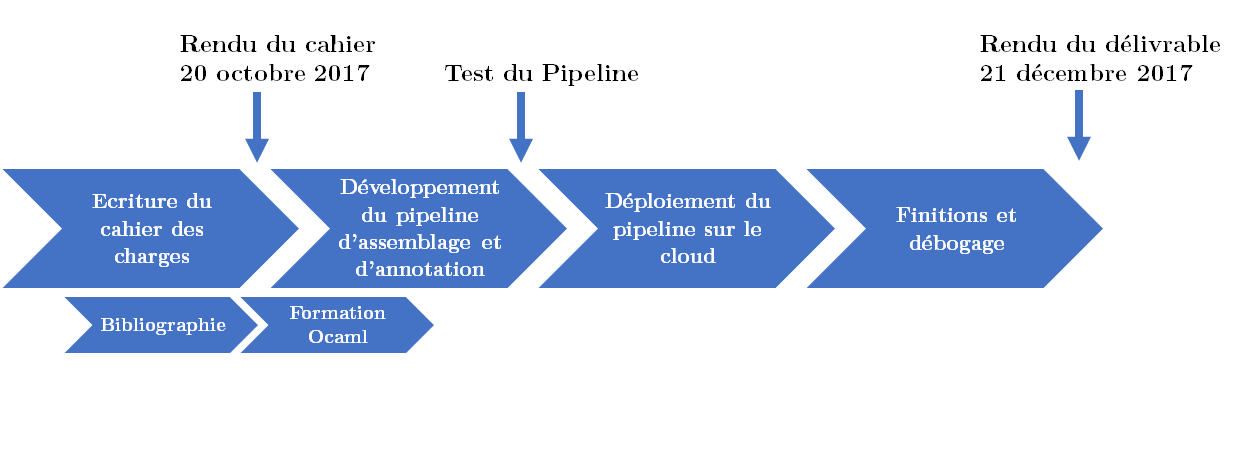
\includegraphics[width=170mm]{images/planning.png}


\subsection{Description des étapes du pipeline et logiciels utilisés}

\subsubsection{Contrôle qualité et trimming des séquences brutes}

\forceindent FASTQScreen : analyse de contamination

\forceindent FASTQC-trimmomatic : contrôle qualité et trimming de lectures courtes

\forceindent LORDEC: contrôle qualité et trimming de lectures courtes 


\subsubsection{Assemblage des lectures}

\forceindent SPAdes \cite{spades}: assembleur conçu pour l'assemblage de novo de génomes bactériens

\forceindent QUAST \cite{gurevich2013quast} : contrôle qualité de l'assemblage (si un génome de référence est disponible)

\subsubsection{Alignement contre génome de référence}

\forceindent BOWTIE2 \cite{langmead2012fast}: aligneur de reads longs contre un génome de référence indexé

\subsubsection{Annotation du génome}

\forceindent ORFinder : détection de gènes de novo

\forceindent BLAST \cite{camacho2009blast+}: annotation comparative et détection de gènes homologues

\forceindent PROKKA : annotation de génomes procaryotes

\subsection{Plan d'assurance qualité}

Pour s’assurer de la qualité du pipeline d’assemblage/annotation, il sera testé sur un jeu de données test de séquençage d’une espèce bactérienne bien annotée dans les bases de données. A priori, les données d’Escherichia coli seront utilisée. Un jeu de données de séquençage Illumina devra être trouvé.


\subsection{Responsabilités}
\textbf{Maîtres d'ouvrage}

Philippe Veber et Stéphane Delmotte (LBBE) sont les maîtres d'ouvrage de ce projet. Les contraintes de temps sont imposées par le Master 2 Bioinformatique de l’université Lyon 1.

\textbf{Maîtres d'oeuvre}

Les quatres étudiants concernés par le projet sont maîtres d’oeuvre, à savoir Lucía Castro García, Cécile Hilpert, Sumaira Javaid et Krystian Valenducq.

  
  \section{Références bibliographiques}
\begin{enumerate}
\item \href{https://www.ncbi.nlm.nih.gov/pmc/articles/PMC4264107/pdf/nihms191018.pdf}{\textbf{Galaxy.}}
 \textbf{Daniel Blankenberg, Gregory Von Kuster, Nathaniel Coraor, Guruprasad Ananda,
Ross Lazarus, Mary Mangan, Anton Nekrutenko, and James Taylor.}
Curr Protoc Mol Biol. 2010 January ; 0 19: Unit–19.1021. Galaxy, a web-based genome analysis tool for experimentalists.\hypertarget{1} \\

\item \href{https://www.ncbi.nlm.nih.gov/pmc/articles/PMC4828917/}{\textbf{MyPro.}}
 \textbf{Yu-Chieh Liao, Hsin-Hung Lin, Amarpreet Sabharwal, Elaine M. Haase, and Frank A. Scannapieco.}
J Microbiol Methods. 2015 Jun; 113: 72–74. MyPro: A seamless pipeline for automated prokaryotic genome assembly and annotation. \\

\item \href{https://www.ncbi.nlm.nih.gov/pubmed/26936607}{\textbf{MEGAnnotator.}}
 \textbf{Lugli GA, Milani C, Mancabelli L, van Sinderen D, Ventura M.}
FEMS Microbiol Lett. 2016 Apr;363(7). MEGAnnotator: a user-friendly pipeline for microbial genomes assembly and annotation.\\

\item \href{https://www.ncbi.nlm.nih.gov/pubmed/20157493}{\textbf{MicroScope.}}
 \textbf{Vallenet D, Engelen S, Mornico D, Cruveiller S, Fleury L, Lajus A, Rouy Z, Roche D, Salvignol G, Scarpelli C, Médigue C.}
Database : the journal of biological databases and curation (Oxford). 2009. MicroScope: a platform for microbial genome annotation and comparative genomics.\\

  
  
  
  
  
  
\end{document}

